% Chapter 2
\chapter[Sample preparation and Experiment Apparatus]{Sample preparation and Experiment Apparatus} % Main chapter title

\label{Chapter2} % Change X to a consecutive number; for referencing this chapter elsewhere, use \ref{ChapterX}

%----------------------------------------------------------------------------------------
%	SECTION 1
%----------------------------------------------------------------------------------------
\section{Sample information}
The nanodiamonds that are used as sample in this project was synthesised from a trinary mixture of naphthalene (C$_{10}$H$_{8}$), highly fluorinated graphite (CF$_{1.1}$) and Tetrakis(trimethylsilyl)silane(C$_{12}$H$_{36}$Si$_{5}$) at a pressure of 8 GPa and a temperature of 1100$^{o}$C. These nanodiamonds carry optically active SiV and NV. The presence of NV is the result of spontaneous doping from the synthesis procedure, more specific, is due to atmospheric nitrogen adsorbed on the surface of naphthalene powder.
\begin{figure}[h]
\centering
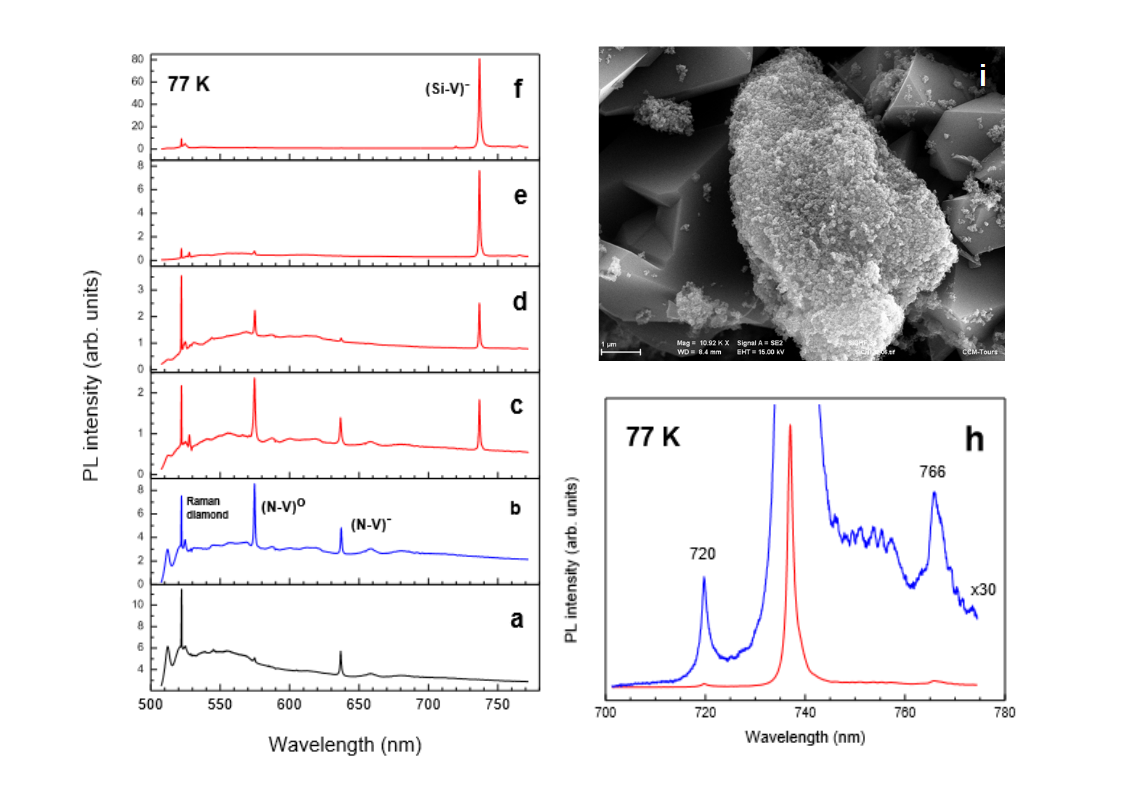
\includegraphics[width=1\linewidth]{Figures/pic/diamondinfo}
\caption{}
\label{fig:diamondinfo}
\end{figure}
\FloatBarrier

To obtain cleaner and more size-refined nanodiamond, the sample was then centrifuged and divided into 4 batches following the condition in table 2.1. in between each step, the residue was re-dispersed in 1ml of microwater.The average size of the nanodiamonds in batch 1 is expected to be the smallest, and the ones in the 4th batch are expected to have the largest size.
\begin {table}[]
\caption {Centrifuging conditions for nanodiamond size selection} \label{tab:title} 
\begin{center}
\begin{tabular}{|c|c|}	
	\hline 
	Batch Number & Centrifuging Condition \\ 
	\hline 
	1 & 2000rpm 1min \\ 
	\hline 
	2 & 1000rpm 1min \\ 
	\hline 
	3 & 500rpm 1min \\ 
	\hline 
	4 & 300rpm 1min \\ 
	\hline 
\end{tabular} 
\end{center}
\end{table}
\section[sample preparation]{sample preparation}
\subsection{preparation of the substrate}
\paragraph{IIa diamond as substrate}

To choose a proper substrate for the nanodiamond sample, a few principles need to be considered.

\paragraph{1.}Low background fluorescence. 
It is always vital to obtain a decent signal to noise ration in any kind of meansurements. As for our case, the emission(fluorescence) from sillicon centers are the target, thus we would love to lower the back ground fluorescence as much as possilble.
\paragraph{2.}Good heat conductivity at low temperature.
From previous calculation done by Uwen Jantzen, we know that the temperature difference $\bigtriangleup T$ between the bottom of the substrate and nanodiamonds(which are spin coated on the surface of the substrate) can be estimate as\newline
$\bigtriangleup T = \frac{\sigma \cdot d \cdot T^{4}}{k} $,
where $\sigma$ is the Stefan–Boltzmann constant, $d$ is the thickness of the substrate and $k$ is the thermal conductivity.
To resolve the fine feature of sillicon vacancy ZPL, we want to characterise the nanodiamond sample at a temperature that is lower than 30K for spectrometer and 10K? for PLE.
\paragraph{3.} No distracting spectral features.
Some misleading peaks from the emission of the substrate would be the least wanted when we want to character a sample spectrally. In many cases, this is related to the raman-scattering of the photons, which highly depends on the crystal structure of the substrate. This scattering process alters the energy of the incident photons by shifts of concrete values and sometime can introduce peaks that are misleading or distracting.
\paragraph{4.}Refractive index. Inam et al calculated the relative emission rate for radiating dipoles near an interface between two dielectrics with FDTD simulation. The result demonstrates that in both of the cases, when the dipole lies prependicular and parallel to the substrate, the emission rate from a interface with lower relative refractive index is always higher than that from a interface with higher relative refractive index. And to increase the emission rate, a substrate with lower refractive index would be prefered.
\paragraph{}Prevously, taking these principles into consideration, my colleges have already ruled out a couple of materials, for instance, glass/quartz(distraction raman shift lines) and Sapphire(also a distracting raman shift line, and impurity induced emission that calls for extra attention when picking the optical filters). Now the temporary choice has landed on IIa type diamond, which has a low impurity density(resulting in low background fluorescence intensity), relatively low refractive index(2,4 to 2,7), good thermal conductivity($\bigtriangleup T = 4,17 \cdot 10^{-2}K$) and a raman shift at 1332$cm^{-1} $ that causes no distraction on our observation.

\paragraph{Focused Ion Beam milling}
In order to make it more convenient to trace the nanodiamonds, markers were curved onto the surface of the IIa type diamond substrate, this work was done by Uwe Jantzen during his master's thesis period. As is shown in the fig.[], the focues ion beam bombards the surface of diamond away and leaves behind markers that are visible in optical microscopy images and SEM images, as well as confocal microscopy images. But the impact of ion may also introduce new defect into the substrate, which will be discussed later.
\FloatBarrier
\begin{figure}[h]
\centering
\includegraphics[width=1\linewidth]{Figures/pic/fib}
\caption{Pictures of markers obtained from FIB, which are placed following the order of numbers. They are visible in optical micrscopes, confocal microscopes as well as SEM   }
\label{fig:20150907sample214spincoated5}
\end{figure}
\FloatBarrier



\subsection{spin-coating of the sample}
\subsubsection{spin-coating theory} 
Spin coating is the method of sample preparing that mainly contains 2 steps:

first, the preading of the liquid. In this step, certain volume of liquid containing the particle that we want to coat with is dropped on the surface of the substrate, driven by the centrifuging force from the rotational movement of the substrate, the liquid would be spread evenly on the surface.

Next, the evaporation of the 'solvent'. While the sample stage rotates, the 'solvent'(In our case is not a real solvent, since nanodiamonds never really desolve.) would evaporate, leaving the particle/molecules that are wanted to be coated on the substrate.

In the spin coating session, a few factors we find important.

1.spin speed: generally the thickness of the liquid layer $t$ is proportional to the inverse of the angular velocity $w$ squared t $\sim$ $\frac{1}{\sqrt{\omega}}$, higher speed would help with forming a more uniform layer, yet this also means a smaller volume of solution, which would lead to lower density of nanodiamonds of the surface. On the other hand, with lower speed, the probability of aggregation would increase, which is also what we want to prevent.

2.volume of the 'solution': larger volume means longer drying time, which would increase the probability of aggregation and losing nanodiamonds, while smaller volume leads towards lower density of nanodiamond and more difficulty when trying to drop it with a pipette. 

3.type of solvent: The type of solvent, viscosity and boiling point are important for the dispersion of nanoparticles inside solution, the spreading of the solution while spin coating and the rate of evaporation.

4.surface condition of the substrate. High contact angle is a obstacle towards the spreading of the solution, high roughness or inappropriate surface group of the substrate can result in poor wettability from the solution.


%-----------------------------------
\subsubsection{Acid cleaning}
To make sure that the NDs dispension can evenly spread and eventually settled on the substrate, a smooth, clean and hydrophilic surface is important.

Acid boiling is a very practicle way of diamond substrate cleaning. As it is called, the diamond will be boiled in a mixture of three strong mineral acids: sulfuric acid, nitric acid and perchloric acid. This mixture has ver strong ability of oxidizing.

After assembling the setup, we initialize the reaction by heating the mixture to a temperature where is mildly bubbles. The substrate would be stay inside the boiling tri-acid mix for 4h. After the acid boiling, the sample should be removed from the flask and rinsed with pure water, after which a rapid blow dry with clean air is conpulsary.
The mixture of strong mineral oxidizing acid can remove most of the adhesions on the surface of diamond substrate , leaving a clean hydrphilic surface. This oxidizing procedure will lead to the formation of carbonyl and carboxyl groups.
One thing that worth notice is that, althought via acid boiling, most of the attachments on the surface can be removed, there is still very high chance to introduce other contaminations from the water, and air while the sample is still wet. So a rapid blow dry after the rinse is highly recommended, and if the acid cleaning is not operated in clean room, it is very important to clean the sample a second time via acetone boiling and ultrasonic bath in the clean room.


\begin{figure}[h]
\centering
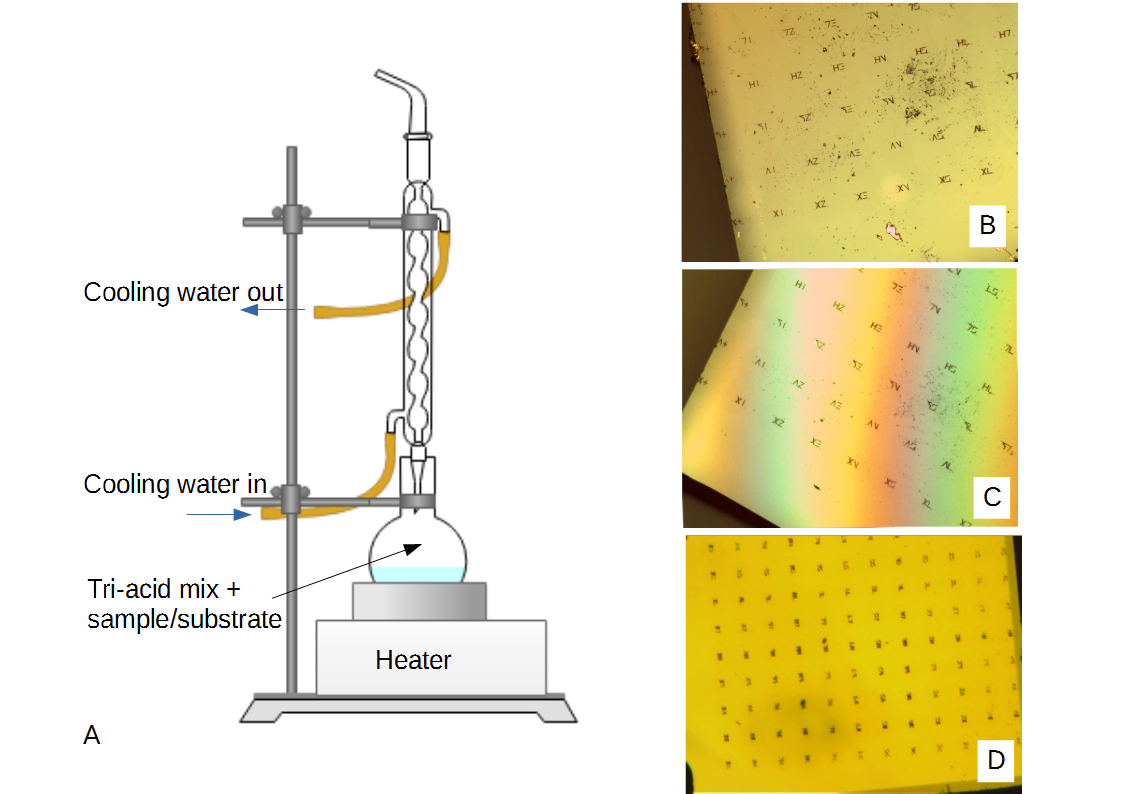
\includegraphics[width=1\linewidth]{Figures/pic/AcidCleaning}
\caption{a) setup up of acid cleaning. b)substrate 207 before cleaning. c) substrate 207 after acid boiling. d) acid cleaned substrate 207 after acetone boiling in the clean room.}
\label{fig:Acid Cleaning}
\end{figure}
 
\subsubsection{spin-coating practice}
Throughout the project, with the help of Andrea Kurz, several combination of these factors had been has been tried out on different samples.

I. 35ul Chloroform with 1ul of nanodiamond, take 2ul of this kind of mixture and drop it on the substrate in one time. The spin speed is 5000rpm and the duration is 40s.(Sample 1506,1507)

II. 30ul Chloroform with 1ul of nanodiamond, 2ul of mixture, apply in one time, 5000rpm and 40s.(Sample 1508,1509)

III. 30ul Choloroform and approximately 120ul of water with 1ul of nanodiamond, 2ul of mixture, apply in one time, 8000rpm and 40s.(Operated on substrate207 and found no SiV$^{-}$ signal later.)

IV. 30ul Choloroform and approximately 120ul of water with 1ul of nanodiamond, 10ul of mixture, apply in 5 times, each time 2ul, after each application, spin with the speed of 5000rpm and  duration of 40s.(sample 1510,1512)

All the 3 methods other than method III produced samples with SiV$^{-}$ containing points of interest. But among them, the method IV offers the highest SiV$^{-}$ density.
 

%-----------------------------------
%	SECTION 2
%-----------------------------------
\section[experiment apparatus]{Experiment Apparatus}

\subsubsection{The initial Setup} 

The setup can be coarsely separate into laser source, confocal microscope(with APD and spectrometer as detector), flow cryostat and vaccum pump 4 parts, they are all sketched in Fig. 2.4.

\begin{figure}[h]
\centering
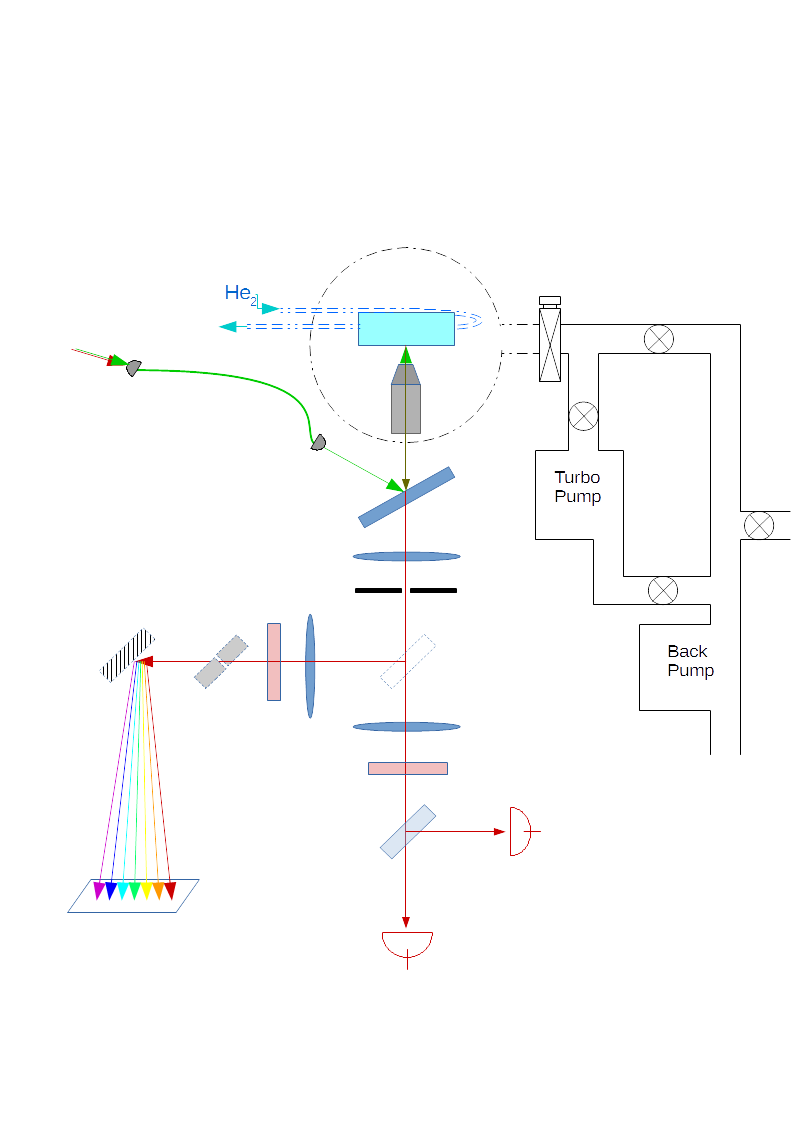
\includegraphics[width=1\linewidth]{Figures/pic/initialsetup}
\caption{A sketch of the initial setup.}
\label{fig:initialsetup}
\end{figure}

While the absorption spectrum shows the highest off resonance absorption around 530nm[need check need find reference paper], the ZPL of silicon vacancy lies around 737nm. Acknowledged of such information, we choose to use green laser of wavelength 532nm as the laser source for photoluminesence spectrum and Titan Sapphire laser with the ability of scanning around 737nm as the laser source of photoluminescence excitation. These two methods will be more detailed written about in the following paragraphs.The lasers are coupled into the same photonic crystal fibre, which guides the beam towards the optical table.

The second part is the confocal microscope, which is a very useful tool for imaging of samples that emits fluorescence, such as SiVs. Compared with fluorescence microscope, as sketched in Fig. 2.5, the confocal microscope uses a pair of convex lens and a pinhole that conjugates to the lens to achieve the increase of resolution and signal to noise ration.
\begin{figure}[h]
	\centering
	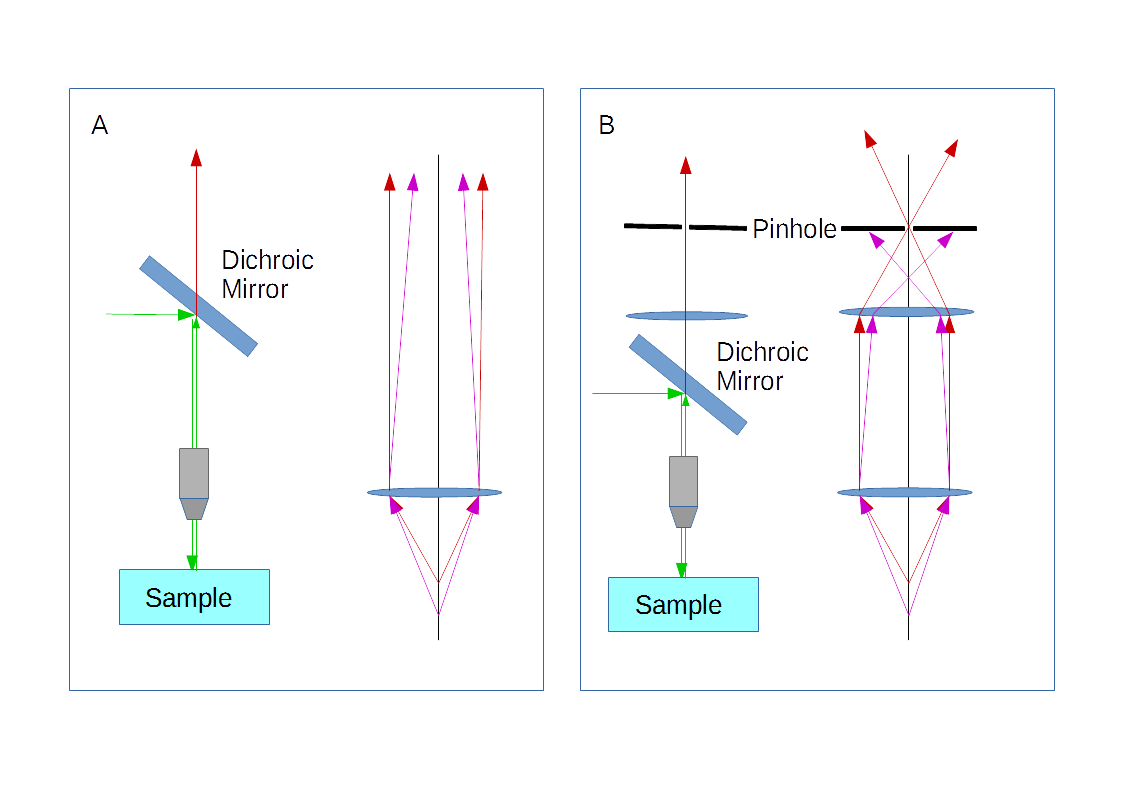
\includegraphics[width=1\linewidth]{Figures/pic/microscope}
	\caption{A)In a typical fluorescence microscope, the back ground fluorescence will also be collected. b)In the confocal microscope, with the help of a lens conjugating pin hole, a large fraction of the fluorescence from non-focus plane will not get through by the pinhole.}
	\label{fig:microscope}
\end{figure}
In the setup, there are two possibilities of signal detection, controlled by a flipping mirror, we can choose to count the photons with a pair of APD, or record the spectrum with a spectrometer.
As the resolution of fine splitting of SiV ZPL needs to be measured in low temperature, the motorized sample stage is placed in a flow cryostat, the objective lens is also inside the cryostat. As the name mentioned, the decrease of temperature in this cryostat is achieved by the flow of cold, boiling liquid Helium, a transfer line connects the Helium dewar and the inlet of the helium cooling circulation inside the cryostat. The sample sits right on the cold finger, with proper method of mounting and substrate, the temperature can be brought to as low as 3.5K(need to check).

To reach cryogenic temperature, it is vital to cut off the heat exchange between the sample and the world out side the cryostat, since air and stainless steel(the material of the cryostat wall) can both conduct heat, a UHV condition need to be meet. In our setup, it is realized by the pumping system of a back pump and a turbo pump. The back pump pre-pumps the pressure until it meets the working condition for turbo pump.

\subsubsection{Methods for characterisation} 
With the mentioned setup, we are able to characterise the sample with following basic methods.


\paragraph{Photoluminescence} 
Photoluminescence detects the emission after the absorption of photons. In our case, we use the 532nm laser to excite the sample, which would bring the SiV$^{-}$ to the second excited state, while the electronic transition between 2 energy levels of the same parity is not allowed, it is possible to conduct the transition between such kind of 2 energy level via the creation and annihilation of phonons, thus it will be the 4 transitions between the first excited state and the ground state that we are expect to record in the spectrum .

The resolving power of a grating in a spectrometer depends on the width of the grating, the centre length to be resolved and the geometry of the use condition. In our setup, a resolution of 16GHz can be achieved, which is capable of observing the 4 line structure in SiV$^{-}$ ZPL, but not enough to resolve a peak with the width of the lifetime limit. 

\paragraph{PLE} When PL excites the sample with a laser of single wavelength to obtain the information about multiple emissions, PLE, on the contrary, excites the sample with various wavelength and monitors the photon emission from the side band to characterise a single transition. The resolution of PLE depends on the resolution of laser, with the Matisse Titan-Sapphire laser(linewidth of 50kHz), it allows us to resolve single electronic transmission in SiV$^{-}$ with life time limited line width, as well as to obtain better signal to noise ratio. 

\paragraph{time resolved PL spectra} It is very inconvenient monitoring the spectral diffusion in the scale of nm with PLE. To help characterise the spectral diffusing behaviour of SiV$^{-}$, we improvised the time-resolved PL spectra. By stacking the sequentially taken spectra in the order of time, we can visualize and estimate the spectral diffusion in a more coarse but convenient way. 
 
Departing from the initial setup, a few alternations have been done during the project, which would be discussed in detail in the following up contents.